\section{基于逻辑回归的集成学习跟踪}

\begin{frame}{工作点1}
    \tableofcontents[sections=\thesection]
\end{frame}

\subsection{算法简介}
\begin{frame}{算法简介}


\begin{block}{}
    基于逻辑回归的集成学习跟踪算法借助简单快速的弱分类器预测目标。为克服弱分类器的性能缺陷,以逻辑回归对其进行选取和集成。该算法以简单特征(Haar-like特征)和粗糙分类器为基础,并显著提高了跟踪的准确性。
    \end{block}
\end{frame}

\subsection{逻辑回归分类器}

\begin{frame}{逻辑回归}

\begin{center}
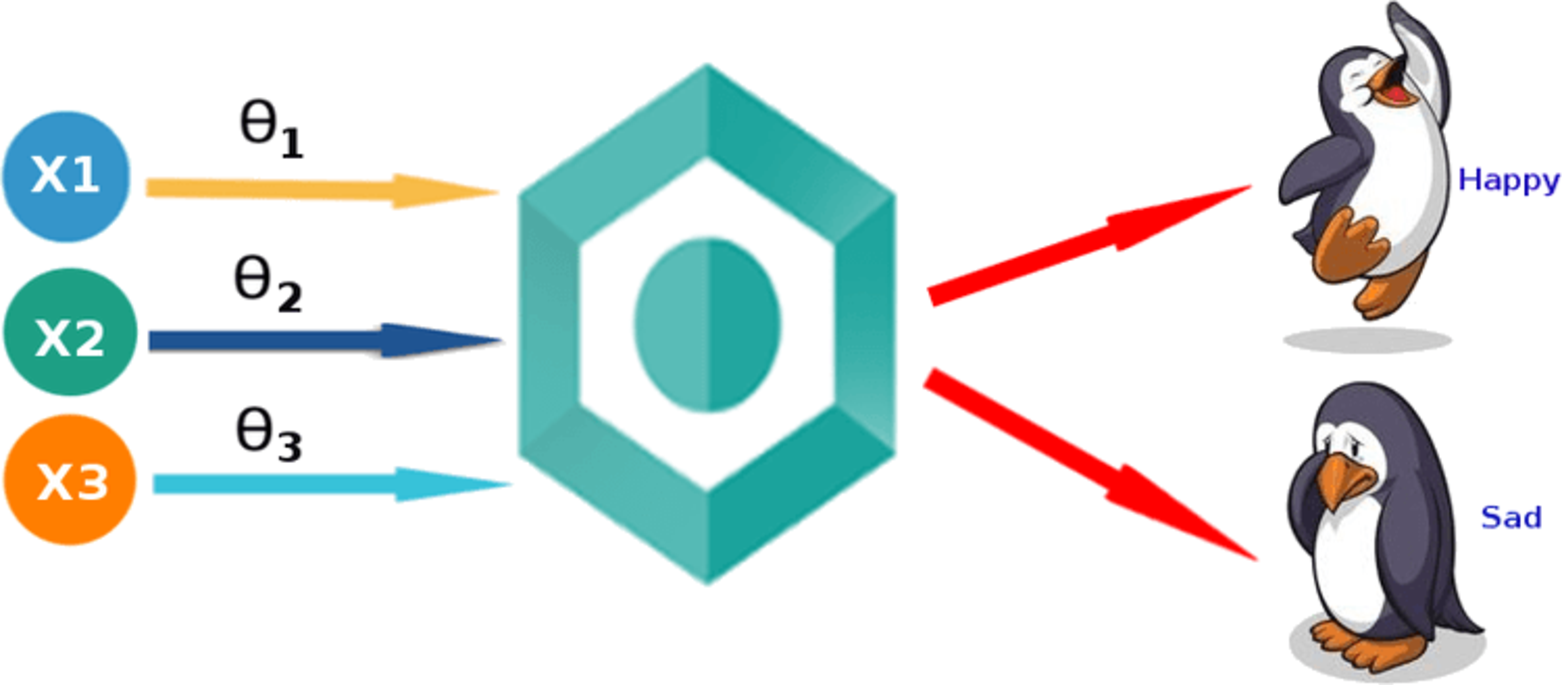
\includegraphics[width =0.5\textwidth,height =0.24\textwidth]{logisticregression.pdf}
\end{center}

逻辑回归为概率型非线性回归模型,是研究分类观察结果与影响因素之间关系的一种多变量分析方法。
~\\
\begin{equation}
P(y|x,w)=\frac{1}{1+\exp(-yx^{T}w) }
\label{eq:LR}
\end{equation}
~\\
其中$ x\in \mathbb{R}^{N} $为一组解释变量或者特征变量,$ y\in \{ -1,+1 \} $为相关联的二进制输出。

\end{frame}
\begin{frame}{模型参数}
逻辑回归试图寻找特征空间中的以法向量$ w\in \mathbb{R}^{N} $为参数的分类超平面,将样本分为两类。
假设给定一个训练或观测样本集合$ x=\{x_{1},x_{2},...,x_{M}\} $与其对应标签$ y=\{y_{1},y_{2},...,y_{M}\} $,模型参数w可通过样本的最大似然估计得到。最大似然估计函数最小化平均损失:
~\\
\begin{equation}
l_{avg}(w)=\frac{1}{M}\sum _{i=1}^{M} \log \left(1+\exp \left( -y_{i} w^{T}x_{i}\right)  \right)
\end{equation}
~\\
\end{frame}

\subsection{弱分类器}

\begin{frame}{Haar-like特征弱分类器}
本章算法使用Haar-like特征。每个弱分类器$ h_{k} $由1个 Haar-like特征$ f_{k} $ 和4个在线估计的参数$ (\mu_{+},\sigma_{+},\mu_{-},\sigma_{-}) $组成。分类器返回对数比值比:
\begin{equation}
\begin{aligned}
    h_{k}(x) &=\log[\frac{P(y=+1|f_{k}(x))}{P(y=-1|f_{k}(x))}]\\
          &=\log[\frac{P(f_{k}(x)|y=+1)P(y=+1)}{P(f_{k}(x)|y=-1)P(y=-1)}]
\end{aligned}
\end{equation}
其中$ P(f_{k}(x)|y=+1) $和$ P(f_{k}(x)|y=-1) $服从正态分布$ N(\mu_{+},\sigma_{+}) $。这里令$ P(y=+1)=P(y=-1) $,根据贝叶斯规则可以求解上述等式。
\end{frame}
\begin{frame}{弱分类器更新}
当弱分类器获得新数据时,使用如下方法进行更新:

\begin{equation}
\mu_{+}\longleftarrow \gamma\mu_{+}+(1-\gamma)\frac{1}{M}\sum_{i|y_{i}=+1}f_{k}(x_{i})
\label{eq:updatMuPosi}
\end{equation}
\begin{equation}
\mu_{-}\longleftarrow \gamma\mu_{-}+(1-\gamma)\frac{1}{M}\sum_{i|y_{i}=-1}f_{k}(x_{i})
\label{eq:updatMuNeg}
\end{equation}
\begin{equation}
\sigma_{+}\longleftarrow \gamma\log\sigma_{+}+(1-\gamma)\sqrt{\frac{1}{M}\sum_{i|y_{i}=+1}(f_{k}(x_{i})-\mu_{+})^{2}}
\label{eq:updatSigmaPosi}
\end{equation}
\begin{equation}
\sigma_{-}\longleftarrow \gamma\log\sigma_{-}+(1-\gamma)\sqrt{\frac{1}{M}\sum_{i|y_{i}=-1}(f_{k}(x_{i})-\mu_{-})^{2}}
\label{eq:updatSigmaNeg}
\end{equation}

\end{frame}

\subsection{逻辑回归集成学习框架}

\begin{frame}{跟踪流程}
\begin{figure}[htbp]
  \centering
  % Requires \usepackage{graphicx}
  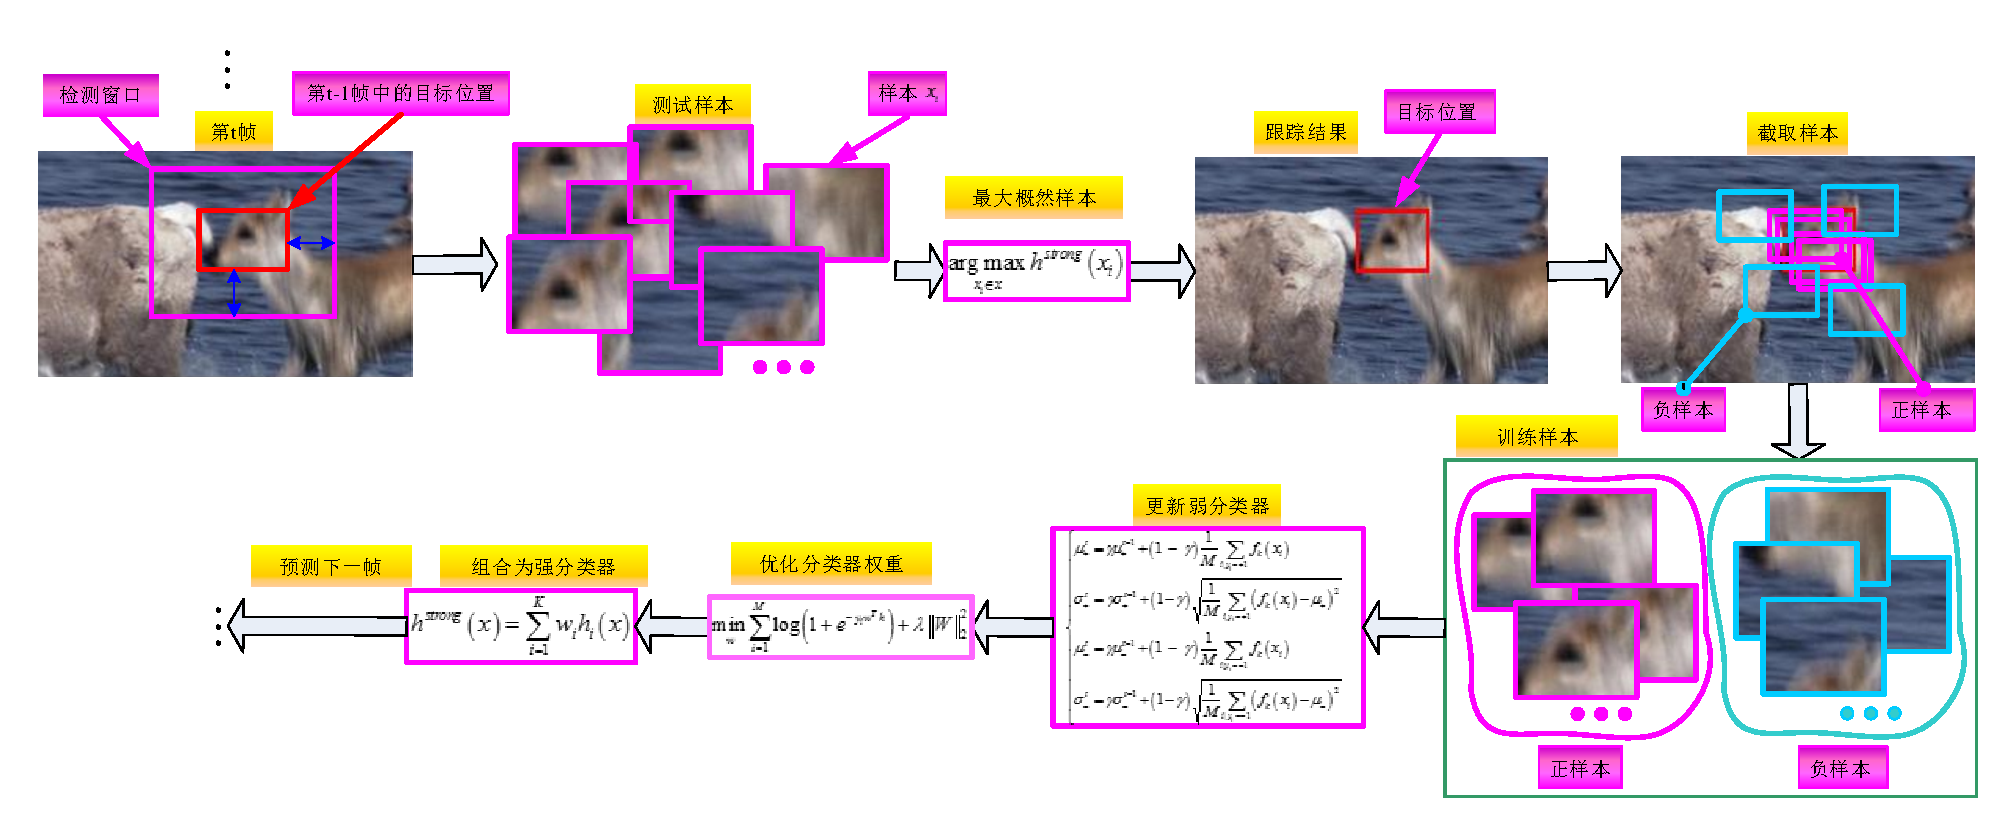
\includegraphics[width=\linewidth]{figures/LR_ArchitecturalStructure.pdf}\\
\caption{逻辑回归集成学习跟踪模型}
\label{fig:LR_ArchitecturalStructure}
\end{figure}

\end{frame}

%\begin{frame}{强分类器预测目标位置}
%当新一帧到来时,算法根据前一帧位置设定测试区域,从中分割出图像块集合。Boosting分类器给出每个图像块是目标的概率值,将概率值最高的图像块认定为目标。
%~\\
%\begin{equation}
%h^{strong}(x)= \sum _{i=1}^{K} w_{i}h_{i}(x)=w^{T}h(x)
%\label{eq:strongClassification}
%\end{equation}
%~\\
%其中$ h_{i}(x),i=1,2,...,K $是弱分类器集合中挑选出的性能较好的K个弱分类器。
%\end{frame}

%\begin{frame}{优化弱分类器权重}
%根据目标位置可以分割出若干图像块作为正负训练样本。在算法中,每一个图像块被视为一个训练样本,并对应一个特征向量。逻辑回归挑选出较好的分类器并赋予合适的权重:
%~\\
 %\begin{equation}
 %\min_{w}\sum _{i=1}^{M} \log \left(1+\exp \left( -y_{i} w^{T}h(x_{i})\right) \right) + \lambda ||w||^{2}_{2}
%\label{eq:optimizeW}
%\end{equation}
%~\\
%其中,$ h(x) = [h_1(x) , h_2(x) , \dots , h_N(x)] $。公式(\ref{eq:optimizeW})通过减少预测标签和真实标签之间的总误差确定弱分类器的权重。

%\end{frame}

\subsection{实验结果}

\begin{frame}{中心位置误差(CLE)}

\begin{table}[!t]
\centering
\renewcommand{\arraystretch}{1.5}
\caption{中心位置误差(像素)}

\begin{adjustbox}{max width=\textwidth}
\begin{tabular}{|c|c|c|c|c|c|c|c|c|c|}
\hline Sequence & CT & CXT & DF & MIL & SCM & Struck & TLD & VTD & Ours\\
\hline Basketball & 89  & 215 & 18 & 92 & 53 & 118 & 269 & \textcolor{red}{6}  & \textcolor{blue}{10} \\
\hline David3     & 89  & 222 & 51 & \textcolor{blue}{30} & 73 & 107 & 281 & 67 & \textcolor{red}{13} \\
\hline Football   & \textcolor{blue}{12}  & 13  & \textcolor{red}{9}  & \textcolor{blue}{12} & 17 & 17  & 14  & 14 & \textcolor{blue}{12} \\
\hline Jogging    & 92  & \textcolor{blue}{6}   & 31 & 96 & 132& 62  & 7   & 83 &  \textcolor{red}{5}\\
\hline Liquor     & 186 & 132 & 221& 142& 99 & 91  & 100 & \textcolor{blue}{60} & \textcolor{red}{57} \\
\hline
\end{tabular}
\end{adjustbox}
\label{tab:LR_CLE}
\end{table}

中心位置误差(Center Location Error, CLE),即检测到的目标框中心与真实目标框中心的平均欧式距离,其值越小代表跟踪结果准确性越高。
\end{frame}

\begin{frame}{重叠精度(OP)}

\begin{table}[!t]
\centering
\renewcommand{\arraystretch}{1.5}
\caption{阈值为0.5的重叠精度(\%)}

\begin{adjustbox}{max width=\textwidth}
\begin{tabular}{|c|c|c|c|c|c|c|c|c|c|}
\hline Sequence & CT & CXT & DF & MIL & SCM & Struck & TLD & VTD & Ours\\
\hline Basketball & 25.93  & 2.48 & 71.59 & 27.45 & 60.28 & 10.21 & 2.48 & \textcolor{red}{92.41}  & \textcolor{blue}{81.51} \\
\hline David3     & 34.92  & 13.89 & \textcolor{blue}{74.21} & 68.25 & 48.02 & 33.73 & 10.32 & 48.41 & \textcolor{red}{84.52} \\
\hline Football   & 78.45 & 65.19  & \textcolor{red}{84.25}  & 73.76 & 57.18 & 66.02  & 41.16  & 76.80 & \textcolor{blue}{78.72} \\
\hline Jogging    & 22.48  & \textcolor{blue}{95.44}   & 21.50 & 22.48 & 21.17& 22.48  & \textcolor{red}{96.74}   & 21.50 &  {95.11}\\
\hline Liquor     & 20.85 & 20.96 & 22.92& 20.10& 32.45 & 40.61  & 56.17 & \textcolor{blue}{57.96} & \textcolor{red}{69.79} \\
\hline
\end{tabular}
\end{adjustbox}
\label{tab:LR_OP}
\end{table}

阈值为0.5的重叠精度(Overlap Precision, OP),即所得目标边界框与真实边界框重叠率超过给定阈值的帧数占总视频的百分比(本文实验中阈值为0.5),其值越大代表跟踪结果越好。
\end{frame}

\newcommand{\mycline}[1]{\tikz{\draw[#1 , line width=3] (0,0) -- (.2,0);}}
\begin{frame}{代表性序列帧及对比算法跟踪结果}

\begin{figure}[htp]
	
	\centering
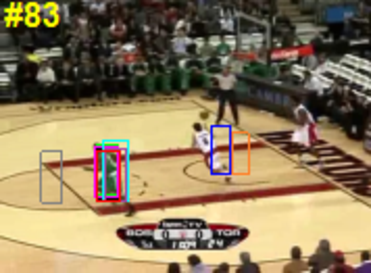
\includegraphics[width=0.31\textheight,height=0.25\textheight]{figures/Figure2a1.pdf}
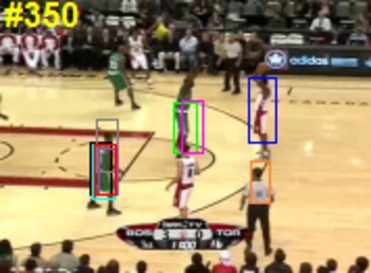
\includegraphics[width=0.31\textheight,height=0.25\textheight]{figures/Figure2a2.pdf}
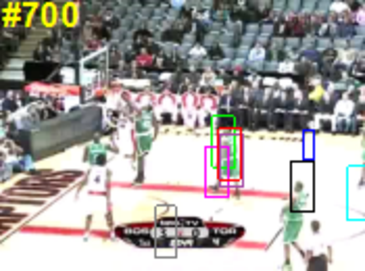
\includegraphics[width=0.31\textheight,height=0.25\textheight]{figures/Figure2a3.pdf}\\

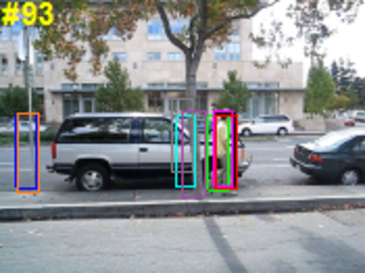
\includegraphics[width=0.31\textheight,height=0.25\textheight]{figures/Figure2b1.pdf}
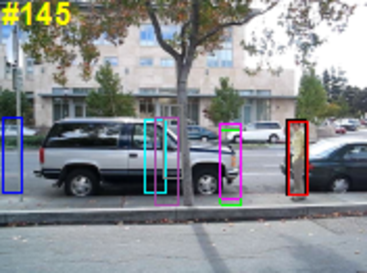
\includegraphics[width=0.31\textheight,height=0.25\textheight]{figures/Figure2b2.pdf}
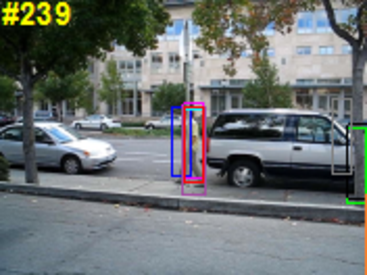
\includegraphics[width=0.31\textheight,height=0.25\textheight]{figures/Figure2b3.pdf}\\

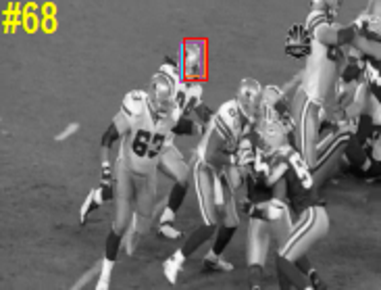
\includegraphics[width=0.31\textheight,height=0.25\textheight]{figures/Figure2c1.pdf}
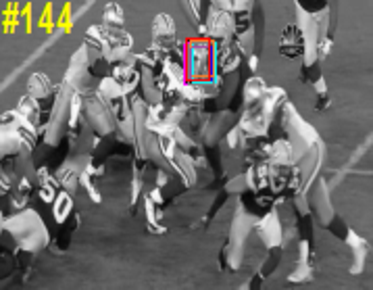
\includegraphics[width=0.31\textheight,height=0.25\textheight]{figures/Figure2c2.pdf}
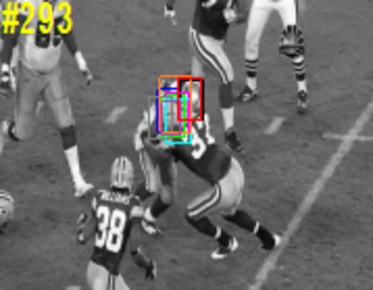
\includegraphics[width=0.31\textheight,height=0.25\textheight]{figures/Figure2c3.pdf}\\

   \mycline{green}CT
   \mycline{blue}CXT
   \mycline{black}DT
   \mycline{pink}MIL
   \mycline{cyan}SCM
   \mycline{gray}Struck
   \mycline{orange}TLD
   \mycline{purple}VTD
   \mycline{red}Ours

%\caption{跟踪过程中代表性序列帧及对比算法跟踪结果}
%\label{fig:LR_trackingResultSample}
\end{figure}

\end{frame}

\begin{frame}{代表性序列帧及对比算法跟踪结果}

\begin{figure}[htp]
	
	\centering
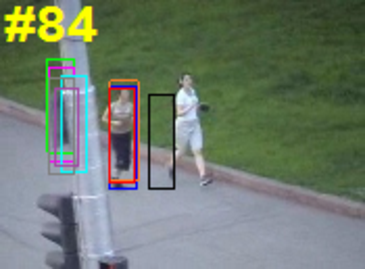
\includegraphics[width=0.31\textheight,height=0.25\textheight]{figures/Figure2d1.pdf}
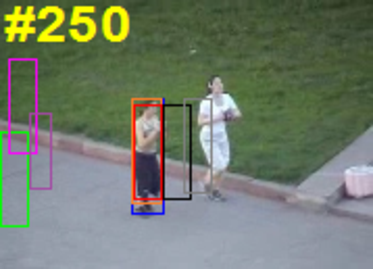
\includegraphics[width=0.31\textheight,height=0.25\textheight]{figures/Figure2d2.pdf}
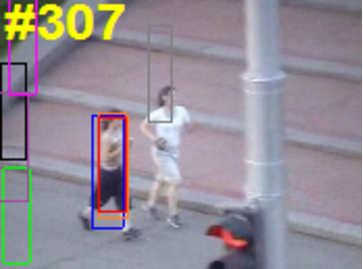
\includegraphics[width=0.31\textheight,height=0.25\textheight]{figures/Figure2d3.pdf}\\

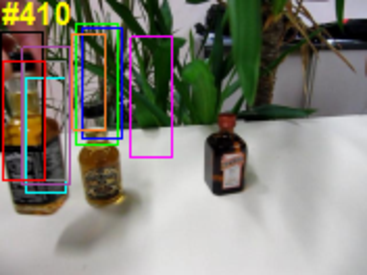
\includegraphics[width=0.31\textheight,height=0.25\textheight]{figures/Figure2e1.pdf}
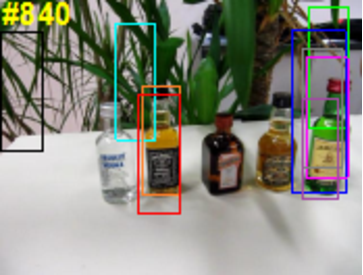
\includegraphics[width=0.31\textheight,height=0.25\textheight]{figures/Figure2e2.pdf}
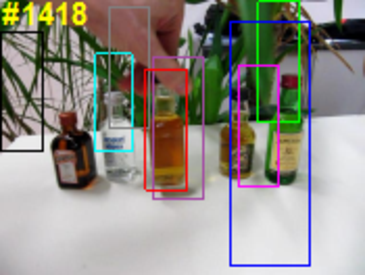
\includegraphics[width=0.31\textheight,height=0.25\textheight]{figures/Figure2e3.pdf}\\

   \mycline{green}CT
   \mycline{blue}CXT
   \mycline{black}DT
   \mycline{pink}MIL
   \mycline{cyan}SCM
   \mycline{gray}Struck
   \mycline{orange}TLD
   \mycline{purple}VTD
   \mycline{red}Ours

%\caption{跟踪过程中代表性序列帧及对比算法跟踪结果}
%\label{fig:LR_trackingResultSample}
\end{figure}

\end{frame}



